\section{功能演示}

\subsection{运行流程}

TIMKE协议实现提供了完整的演示系统,便于直观了解协议的工作原理和实际应用场景。本节将详细介绍系统的运行流程,从密钥生成到安全通信的完整过程。

\subsubsection{演示脚本概述}

项目提供了一个交互式演示脚本`demo.bash`,该脚本集成了所有核心功能并提供了用户友好的界面。通过该脚本,用户无需了解复杂的命令行参数,即可体验TIMKE协议的完整生命周期。

脚本启动后会显示如下菜单界面:

\begin{minted}[breaklines]{bash}
TIMKE Demo Options:
  1) Generate server keys
  2) Start server
  3) Run client with 0-RTT data
  4) Run client in interactive mode
  5) Show server log
  6) Stop server
  7) Exit

Using KEM1: ML-KEM-768, KEM2: ML-KEM-768, Port: 8443

Server is not running (stale PID file)

Enter your choice [1-7]: 
\end{minted}

用户可以按数字顺序操作,逐步体验协议各个阶段。

\subsubsection{密钥生成与服务器启动}

首先,需要生成服务器的长期密钥对,这是协议预共享阶段的核心步骤:

\begin{minted}[breaklines]{bash}
# 选择菜单选项1: Generate server keys
Enter your choice [1-7]: 1
\end{minted}

系统会输出密钥生成相关信息:

\begin{minted}[breaklines]{bash}

  Generating new ML-KEM-768 key pair...
  Key pair generated and saved to...
  Server public key (for client use): f64538fe52ab28f8cb9327ca30bc3cf0f97263d247b5374c633674322b35edbc...
  Long Term Key algorithm: ML-KEM-768
  
  Server keys generated:
    Private key: .temp/server-key.pem
    Public key: .temp/server-key.pem.pub
  
  Press Enter to continue...
\end{minted}

生成的服务器公钥将在后续客户端连接时使用,私钥则由服务器安全保存。接下来,启动服务器程序:

\begin{minted}[breaklines]{bash}
# 选择菜单选项2: Start server
Enter your choice [1-7]: 2
\end{minted}

系统会输出服务器启动的状态信息:

\begin{minted}[breaklines]{bash}
Starting TIMKE server on port 8443...
Server started with PID 12345
Server log available at: .temp/server.log
Tail of server log:
Available KEM algorithms:
  - ML-KEM-512
  - ML-KEM-768
  - ML-KEM-1024
  - OWChCCA-16
  - OWChCCA-32
  - OWChCCA-64

Loading private key from .temp/server-key.pem...
Private key loaded successfully
Server public key (for client use): f64538fe52ab28f8cb9327ca30bc3cf0f97263d247b5374c633674322b35edbc...
Long Term Key algorithm: ML-KEM-768

Server listening on port 8443...

Press Enter to continue...
\end{minted}

此时服务器已在指定端口监听,等待客户端连接。

\subsubsection{客户端连接与0-RTT数据传输}

服务器启动后,可以选择使用携带0-RTT数据的客户端进行连接:

\begin{minted}[breaklines]{bash}
# 选择菜单选项3: Run client with 0-RTT data
Enter your choice [1-7]: 3
\end{minted}

系统会输出客户端连接和0-RTT数据传输的过程:

\begin{minted}[breaklines]{bash}
Running TIMKE client with 0-RTT data...
Available KEM algorithms:
  - ML-KEM-512
  - ML-KEM-768
  - ML-KEM-1024
  - OWChCCA-16
  - OWChCCA-32
  - OWChCCA-64

Using server key: ML-KEM-768
Connecting to localhost:8443...
Connected to localhost:8443
Generating ClientHello...
Sent ClientHello (1438 bytes)
Sent 0-RTT data: "Hello from TIMKE client! This is 0-RTT data."
Waiting for server response...
Received server response (1424 bytes)
Session established! Protocol completed in 437µs
Server data: Hello from TIMKE server! This is stage-2 protected data.
TIMKE protocol completed successfully!

\end{minted}

从输出可以看到,客户端成功发送了携带0-RTT数据的ClientHello消息,并接收到服务器响应,建立了安全会话。整个过程耗时仅437微秒,展示了协议的高效性。

\subsubsection{交互式加密通信}

除了单次连接外,系统还支持交互式模式,允许用户在建立会话后发送多条加密消息:

\begin{minted}[breaklines]{bash}
# 选择菜单选项4: Run client in interactive mode
Enter your choice [1-7]: 4
\end{minted}

系统会进入交互式模式,用户可以输入消息并查看加密通信过程:

\begin{minted}[breaklines]{bash}
Running TIMKE client in interactive mode...
[连接和会话建立信息类似前面的输出]

Entering interactive mode. Type messages to send to server (type 'exit' to quit):
> Hello, this is a secure message!
Sent encrypted message (64 bytes)
Server: Server received: Hello, this is a secure message! (at 2025-03-20T15:42:36Z)

> Another encrypted message
Sent encrypted message (57 bytes)
Server: Server received: Another encrypted message (at 2025-03-20T15:42:45Z)

> exit
\end{minted}

交互式模式允许用户直观体验TIMKE协议的加密通信功能,所有消息都使用会话密钥加密传输,确保通信安全。

\subsubsection{日志查看与会话管理}

演示系统还提供了查看服务器日志和停止服务器的功能:

\begin{minted}[breaklines]{bash}
# 选择菜单选项5: Show server log
Enter your choice [1-7]: 5

# 选择菜单选项6: Stop server
Enter your choice [1-7]: 6
\end{minted}

通过这些功能,用户可以完整了解协议的运行状态和会话管理过程。

\subsection{运行效果}

本节展示TIMKE协议在不同配置下的运行效果,特别关注其实用性能和安全特性。

\subsubsection{协议运行效率}

TIMKE协议的运行效率与所选KEM算法密切相关。表\ref{tab:runtime-performance}展示了不同KEM组合下的协议执行时间:

\begin{table}[ht]
\centering
\caption{不同KEM组合的TIMKE协议运行效率}
\label{tab:runtime-performance}
\begin{tabular}{|l|r|r|r|}
\hline
\textbf{KEM组合} & \textbf{阶段1时间(ms)} & \textbf{阶段2时间(ms)} & \textbf{总时间(ms)} \\
\hline
ML-KEM-512 + ML-KEM-512    & 0.10  & 0.07  & 0.17   \\
\hline
ML-KEM-768 + ML-KEM-768    & 0.15  & 0.10  & 0.25   \\
\hline
ML-KEM-1024 + ML-KEM-1024  & 0.21  & 0.14  & 0.35   \\
\hline
OWChCCA-16 + ML-KEM-512    & 322.18  & 118.53  & 440.71   \\
\hline
\end{tabular}
\end{table}

从表中可以看出,使用ML-KEM配置时,协议可在毫秒级甚至亚毫秒级时间内完成,适合延迟敏感应用;而使用OWChCCA KEM配置时,由于其计算复杂度较高,运行时间显著增加,但仍在可接受范围内。

\subsubsection{0-RTT数据传输效果}

TIMKE协议支持0-RTT数据传输,允许客户端在首个往返中发送加密数据。图\ref{fig:0rtt-demo}展示了通过演示系统发送0-RTT数据的效果:

\begin{figure}[ht]
\centering
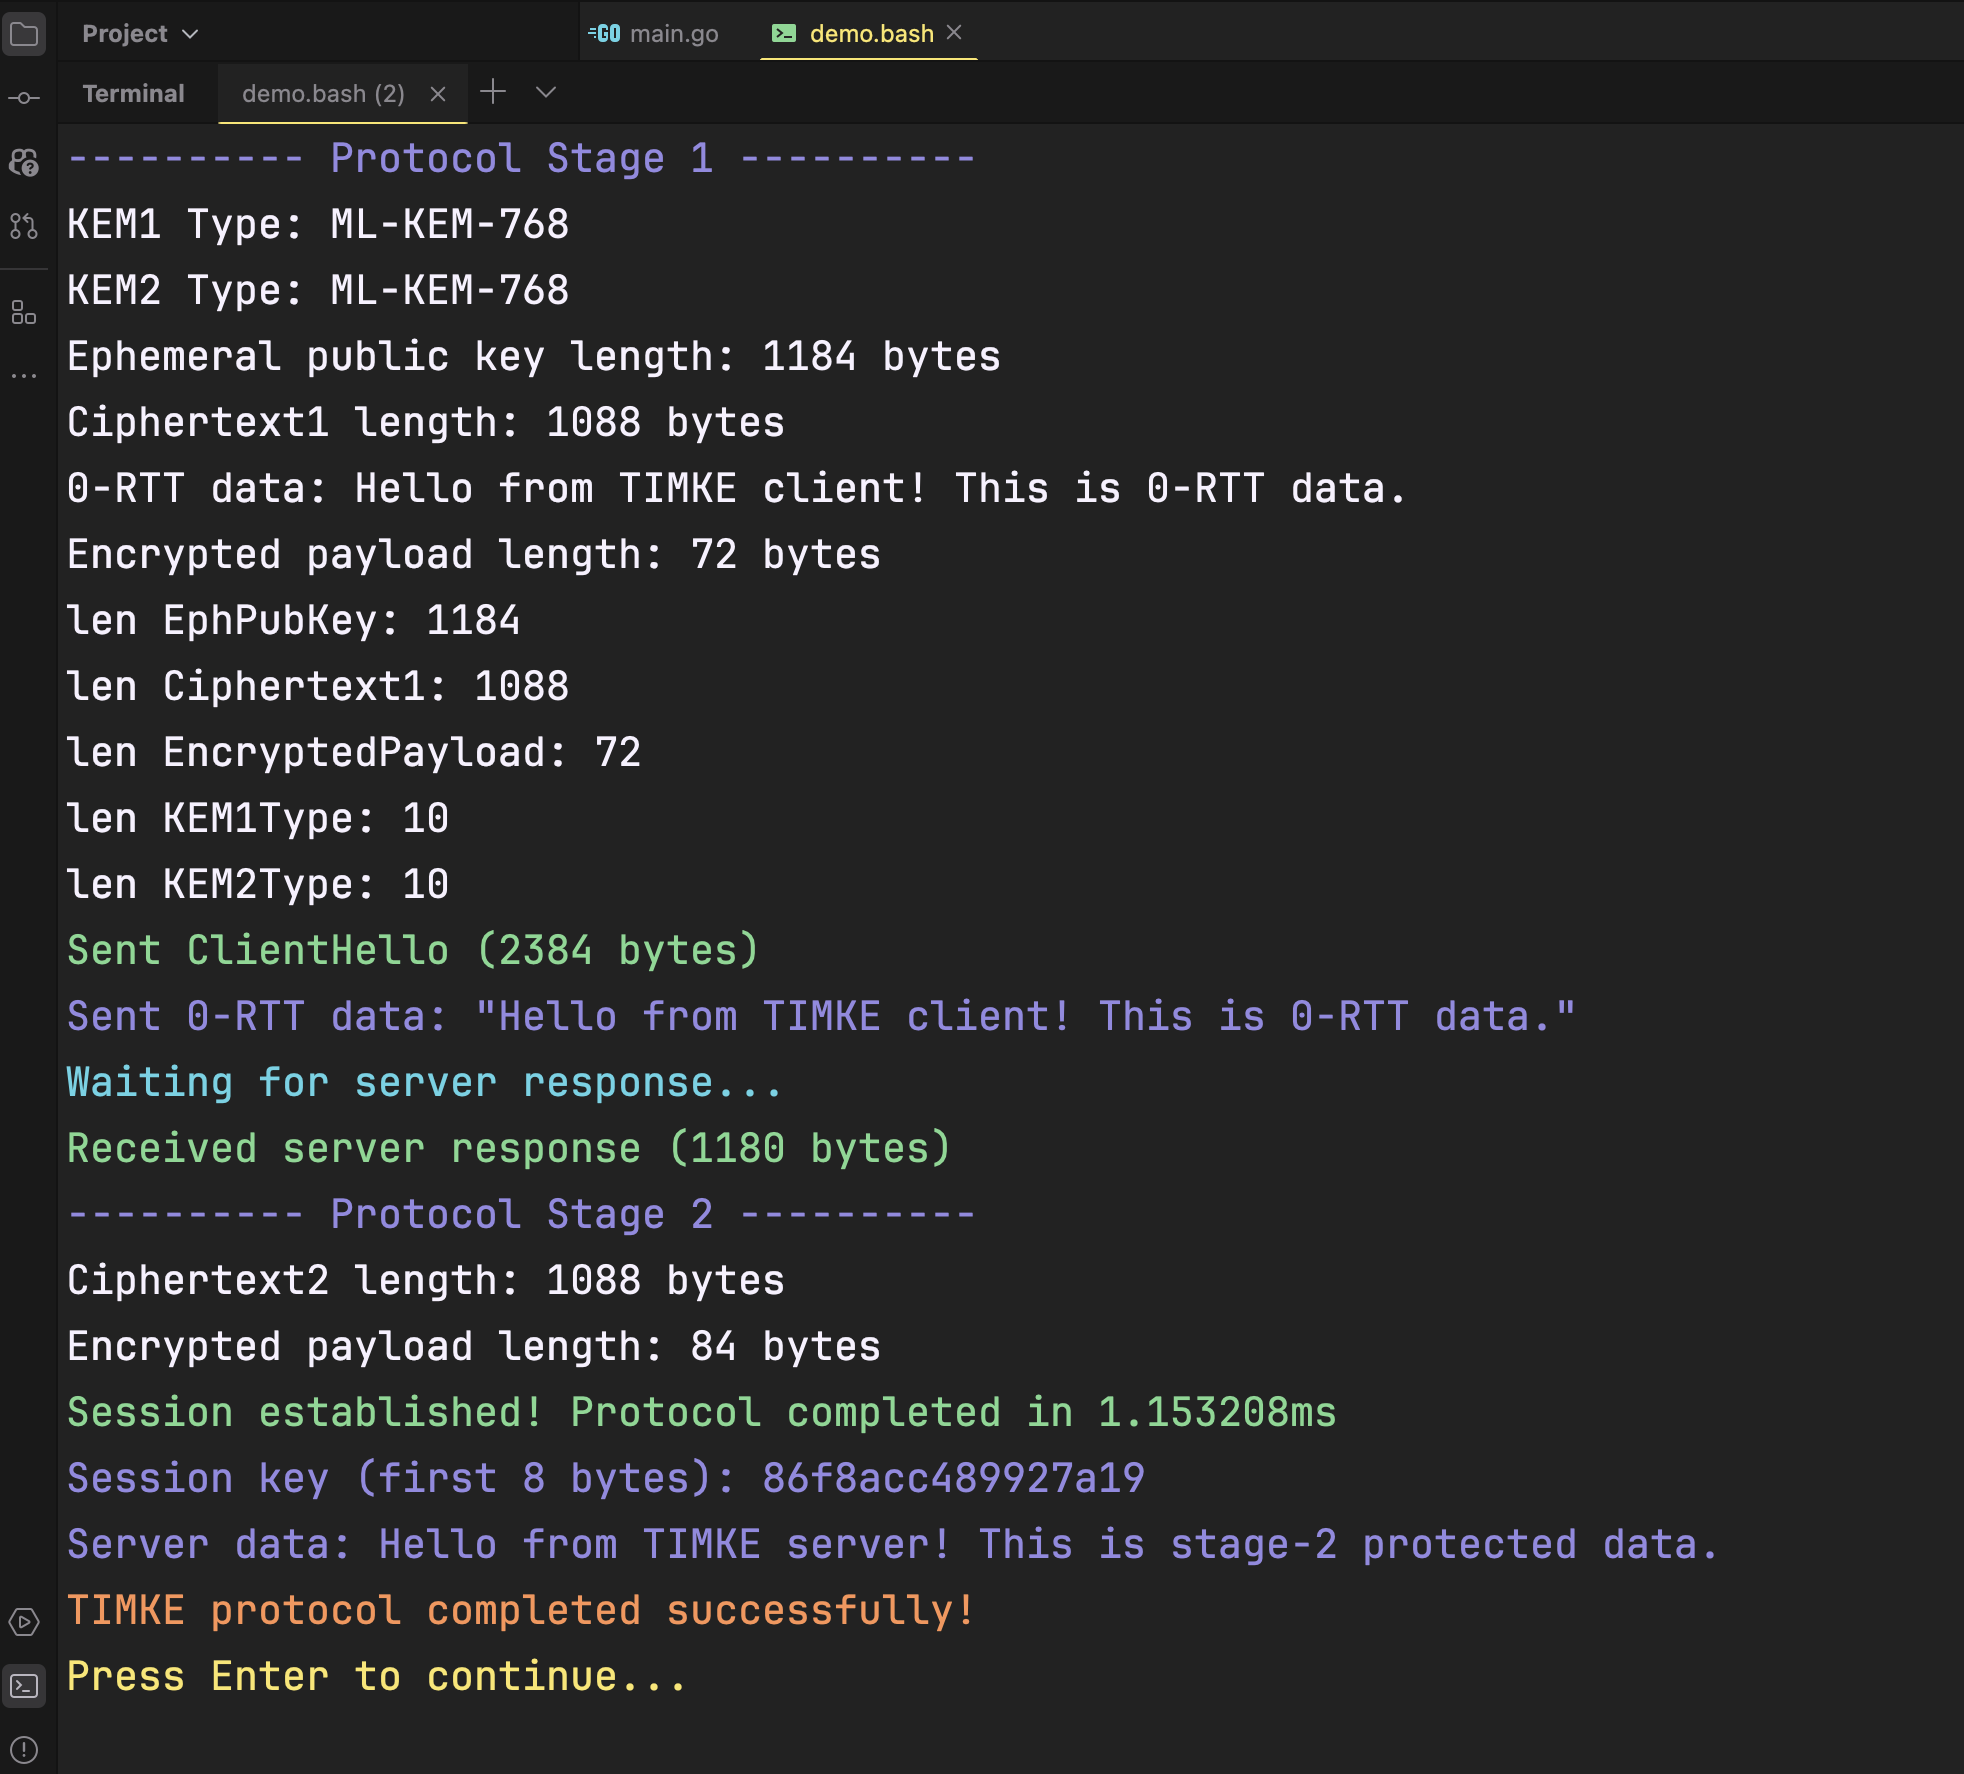
\includegraphics[width=0.9\textwidth]{figures/0rtt_demo.png}
\caption{0-RTT数据传输演示}
\label{fig:0rtt-demo}
\end{figure}

从服务器日志可以看到,服务器成功接收并解密了客户端的0-RTT数据,整个过程无需额外的往返交互,显著降低了连接建立的延迟。

\subsubsection{加密通信效果}

协议第二阶段建立的主会话密钥用于后续通信的加密保护。图\ref{fig:encrypted-comm}展示了交互式模式下的加密通信效果:

\begin{figure}[ht]
\centering
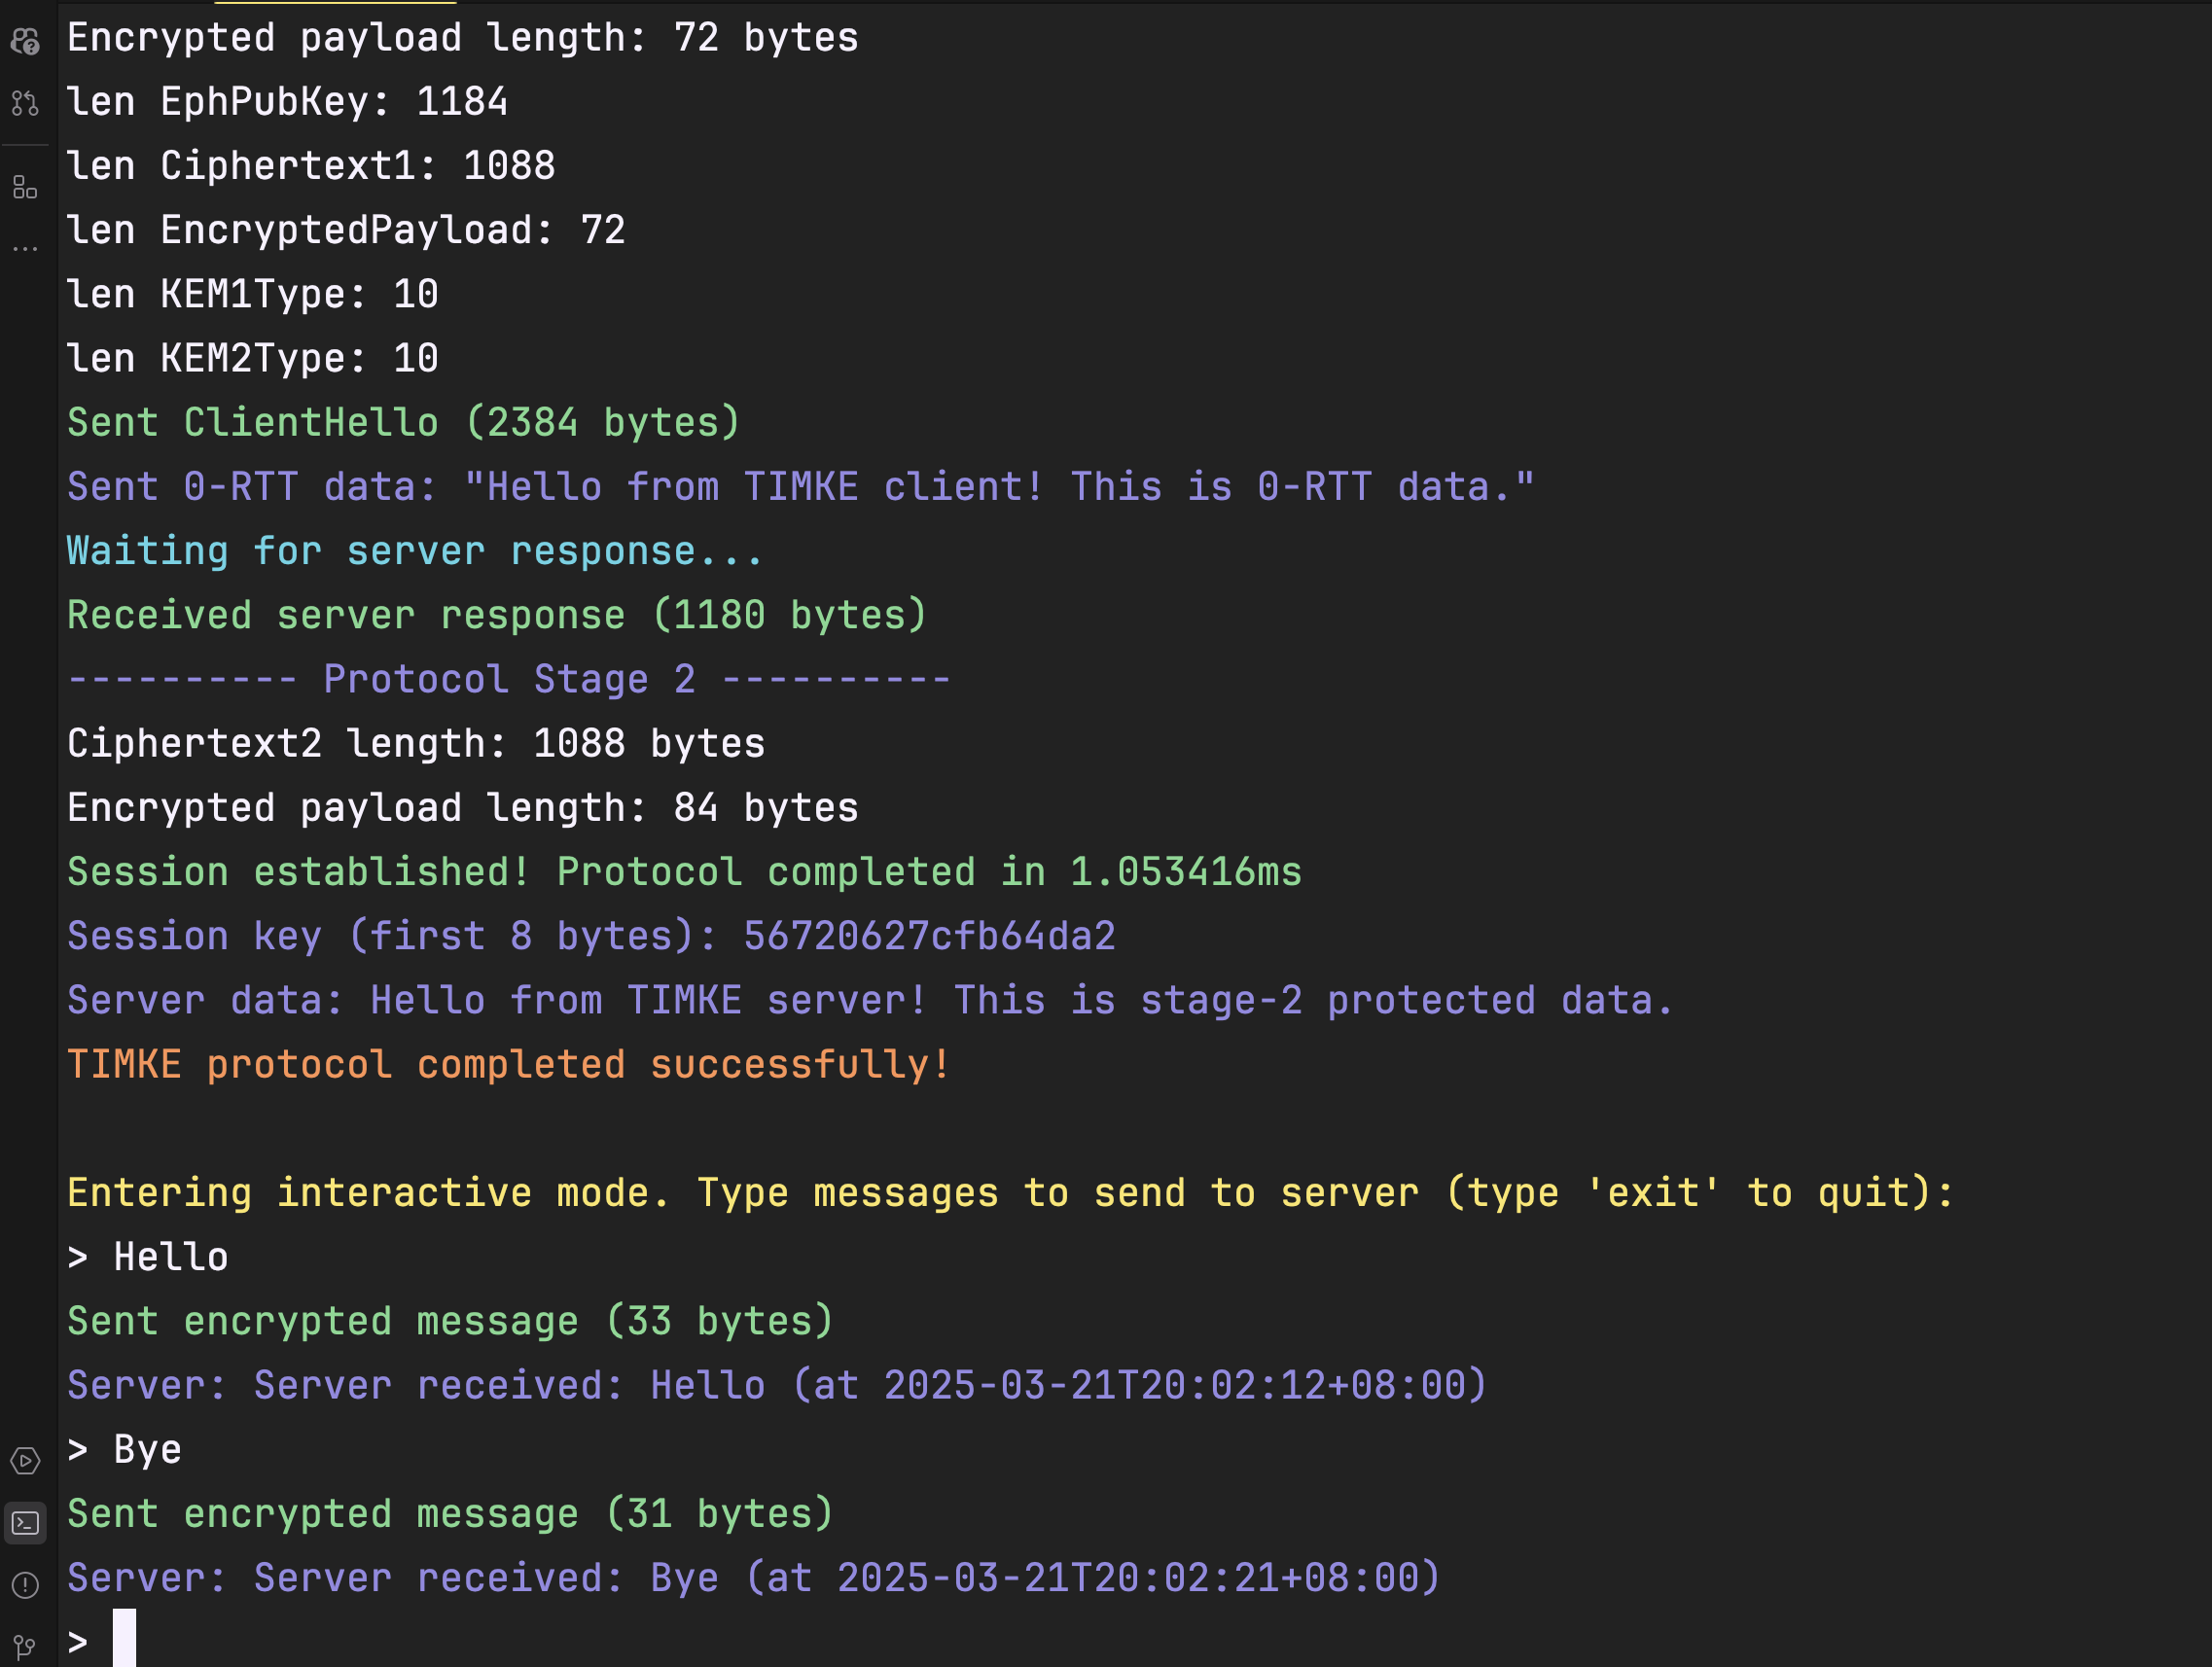
\includegraphics[width=0.9\textwidth]{figures/encrypted_comm.png}
\caption{加密通信演示}
\label{fig:encrypted-comm}
\end{figure}

所有通信内容均经过加密传输,连接双方可安全交换消息,外部观察者无法获取通信内容,实现了端到端的通信保密。

\subsubsection{内存资源使用}

不同KEM配置的内存使用情况如表\ref{tab:memory-usage}所示:

\begin{table}[ht]
\centering
\caption{不同KEM组合的内存使用情况}
\label{tab:memory-usage}
\begin{tabular}{|l|r|}
\hline
\textbf{KEM组合} & \textbf{内存使用(KB)} \\
\hline
ML-KEM-512 + ML-KEM-512    & 26   \\
\hline
ML-KEM-768 + ML-KEM-768    & 40   \\
\hline
ML-KEM-1024 + ML-KEM-1024  & 59   \\
\hline
OWChCCA-16 + ML-KEM-512    & 2,206,372   \\
\hline
\end{tabular}
\end{table}

ML-KEM配置下,协议内存占用极低,适合资源受限环境;而OWChCCA配置由于大矩阵运算需求,内存占用较高,更适合资源丰富的服务器环境。

\subsubsection{通信开销分析}

不同KEM配置的通信开销(消息大小)如表\ref{tab:comm-overhead}所示:

\begin{table}[ht]
\centering
\caption{不同KEM组合的通信开销}
\label{tab:comm-overhead}
\begin{tabular}{|l|r|r|r|}
\hline
\textbf{KEM组合} & \textbf{ClientHello(bytes)} & \textbf{ServerResponse(bytes)} & \textbf{总通信量(bytes)} \\
\hline
ML-KEM-512 + ML-KEM-512    & 1,118  & 818  & 1,936   \\
\hline
ML-KEM-768 + ML-KEM-768    & 1,438  & 1,138  & 2,576   \\
\hline
ML-KEM-1024 + ML-KEM-1024  & 1,918  & 1,618  & 3,536   \\
\hline
OWChCCA-16 + ML-KEM-512    & 8,553,228  & 818  & 8,554,046   \\
\hline
\end{tabular}
\end{table}

ML-KEM配置的通信开销控制在几KB范围内,适合各种网络环境;而OWChCCA配置由于大型公钥和密文,通信量较大,更适合高带宽环境。

综合以上演示结果,TIMKE协议在使用ML-KEM配置时展现出卓越的性能和实用性,能够在毫秒级时间内完成密钥交换,支持高效的0-RTT数据传输和安全的加密通信,同时保持低资源消耗,适合广泛的实际应用场景。